\documentclass{article}
\usepackage[utf8]{inputenc}
\usepackage[left=1.0cm,right=1.0cm, top=1.5cm, bottom=1.5cm]{geometry}
\usepackage{graphicx}
\usepackage{graphics}
\usepackage{caption}
\usepackage{float}
\usepackage{amsmath}
\usepackage{amssymb}
\usepackage{amsthm}
\usepackage{listings}
\usepackage{mathtools}
\usepackage{hyperref}

% Align all equations left:
\documentclass[fleqn]{article} 


% Sets and quantifiers
\newcommand{\R}{\mathbb{R}\;}
\newcommand{\Q}{\mathbb{Q}\;}
\newcommand{\N}{\mathbb{N}\;}
\newcommand{\nin}{n \in \mathbb{N}}
\newcommand{\fa}{\;\forall\;}
\newcommand{\ex}{\;\exists\;}
\newcommand{\nex}{\;\nexists\;}

% Sequences
\newcommand{\seq}[1]{\{#1\}}
\newcommand{\seqx}{\seq{x_n}}
\newcommand{\seqy}{\seq{y_n}}
\newcommand{\seqs}{\seq{s_n}}

% Subsequences
\newcommand{\seqxni}{\seq{x_{n_i}}}
\newcommand{\seqyni}{\seq{y_{n_i}}}
\newcommand{\xni}{x_{n_i}}
\newcommand{\yni}{y_{n_i}}
\newcommand{\xnij}{x_{n_{i_j}}}
\newcommand{\ynij}{y_{n_{i_j}}}
\newcommand{\seqxnij}{\seq{x_{n_{i_j}}}}
\newcommand{\seqynij}{\seq{y_{n_{i_j}}}}

% Such that
\newcommand{\st}{\;\text{such that}\;}

% Machine Vision
\newcommand{\xhat}{\hat{\mathbf{x}}}
\newcommand{\yhat}{\hat{\mathbf{y}}}
\newcommand{\zhat}{\hat{\mathbf{z}}}
\newcommand{\nhat}{\hat{\mathbf{n}}}
\newcommand{\shat}{\hat{\mathbf{s}}}
\newcommand{\rhat}{\hat{\mathbf{r}}}
\newcommand{\vhat}{\hat{\mathbf{v}}}
\newcommand{\hatvector}[1]{\hat{\mathbf{1}}}
\newcommand{\mb}[1]{\mathbf{#1}}
\newcommand{\der}[2]{\frac{d #1}{d #2}}
\newcommand{\dder}[2]{\frac{d^2 #1}{d #2^2}}
\newcommand{\pd}[2]{\frac{\partial #1}{\partial #2}}
\newcommand{\pdd}[2]{\frac{\partial^2 #1}{\partial #2^2}}
\newcommand\numberthis{\addtocounter{equation}{1}\tag{\theequation}}

% Plot functions
\usepackage{tikz}
\usepackage{pgfplots}
\usetikzlibrary{datavisualization}


% lim, limsup, liminf
\newcommand{\limn}{\text{lim}_{n \rightarrow \infty}}
\newcommand{\limi}{\text{lim}_{i \rightarrow \infty}}
\newcommand{\limj}{\text{lim}_{j \rightarrow \infty}}
\newcommand{\limsupn}{\limsup_{n \rightarrow \infty}}
\newcommand{\liminfn}{\liminf_{n \rightarrow \infty}}

% Parallel symbols
\newcommand{\parallelsum}{\mathbin{\!/\mkern-5mu/\!}}


% Custom for absolute value
\delimitershortfall-1sp
\newcommand\abs[1]{\left|#1\right|}

% Reference and hyperlink
\newcommand{\source}[1]{\href{#1}{(\textbf{Source})}}

% Use for define equals
\newcommand{\delteq}{\overset{\Delta}{=}}

% For nicer fonts
\usepackage{eucal}

% For Dreamer Paper
\newcommand{\stau}{s_{\tau}}
\newcommand{\expect}[1]{\mathbb{E}_{#1}}
\newcommand{\indep}{\perp \!\!\! \perp}


\title{6.801/6.866: Machine Vision, Lecture 11}
\author{Professor Berthold Horn, Ryan Sander, Tadayuki Yoshitake \\
        MIT Department of Electrical Engineering and Computer Science \\ 
        Fall 2020}
\date{}
\begin{document}

\maketitle
These lecture summaries are designed to be a review of the lecture.  Though I do my best to include all main topics from the lecture, the lectures will have more elaborated explanations than these notes.  Therefore, if you're looking for the most rigorous review and treatment of these topics, we encourage you to rewatch the lecture videos.  With that said, we hope these summaries are beneficial for your learning.  If you have any feedback for these lecture summaries, please submit it \textbf{\href{https://forms.gle/itCUtP4AubAbtwQT9}{here}}.
\section{Lecture 11: Edge detection, Subpixel Position, CORDIC, Line Detection, (US 6,408,109)}
In this lecture, we will introduce some discussion on how patents work, their stipulations, and make our discussion explicit by looking at a patent case study with sub-pixel accuracy edge detection.  You can find the patent document on Stellar as well under ``Materials" $\rightarrow$ ``US patent 6,408,109".
\subsection{Background on Patents}
We will begin with some fun facts about industrial machine vision:
\begin{itemize}
    \item Integrated circuit boards cannot be manufactured without machine vision
    \item Pharmaceutical chemicals also cannot be manufactured without machine vision
\end{itemize}
How do entrepreneurs and industrial companies ensure their inventions are protected, while still having the chance to disseminate their findings with society?  This is done through \textbf{patents}.  Patents:
\begin{itemize}
    \item Can be thought of as a ``contract with society" - you get a limited monopoly on your idea, and in turn, you publish the technical details of your approach.
    \item Can help to reduce litigation and legal fees.
    \item Can be used by large companies as ``ammunition" for ``patent wars".
\end{itemize}
Some ``rules" of patents:
\begin{itemize}
    \item No equations are included in the patent (no longer true)
    \item No greyscale images - only black and white
    \item Arcane grammar is used for legal purposes - ``comprises", ``apparatus", ``method", etc.
    \item References of other patents are often included - sometimes these are added by the patent examiner, rather than the patent authors
    \item Most patents end with something along the lines of ``this is why our invention was necessary" or ``this is the technical gap our invention fills"
    \item Software is not patentable - companies and engineers get around this by putting code on hardware and patenting the ``apparatus" housing the code.
    \item It is also common to include background information (similar to related literature in research).
\end{itemize}
Now that we have had a high-level introduction to patents, let us turn to focus on one that describes an apparatus for sub-pixel accuracy edge finding.
\subsection{Patent Case Study: Detecting Sub-Pixel Location of Edges in a Digital Image}
To put this problem into context, consider the following:
\begin{itemize}
    \item Recall that images typically have large regions of uniform/homogeneous intensity
    \item Image arrays are very memory-dense.  A more sparse way to transfer/convey information about an image containing edges is to use the locations of edges as region boundaries of the image.  This is one application of edge finding.
    \item This patent achieves 1/40$^\text{th}$ pixel accuracy. 
\end{itemize}
This methodology and apparatus seeks to find edges of objects in digital images at a high sub-pixel accuracy level.  To do so, the authors leverage different detectors, or kernels.  These kernels are similar to some of the computational molecules we have already looked at in this course:
\begin{itemize}
    \item \textbf{Robert's Cross}: This approximates derivatives in a coordinate system rotated 45 degrees $(x', y')$.  The derivatives can be approximated using the $K_{x'}$ and $K_{y'}$ kernels:
    \begin{align*}
        &\pd{E}{x'} \rightarrow K_{x'} = \begin{bmatrix}0 & -1 \\ -1 & 0\end{bmatrix} \\
        &\pd{E}{y'} \rightarrow K_{y'} = \begin{bmatrix}1 & 0 \\ 0 & -1\end{bmatrix} &&
    \end{align*}
    \item \textbf{Sobel Operator}: This computational molecule requires more computation and it is not as high-resolution.  It is also more robust to noise than the computational molecules used above:
    \begin{align*}
        &\pd{E}{x} \rightarrow K_{x} = \begin{bmatrix}-1 & 0 & 1 \\ 
                                                       2 & 0 & 2 \\ 
                                                       -1 & 0 & 1
                                        \end{bmatrix} \\
        &\pd{E}{y} \rightarrow K_{y} = \begin{bmatrix}-1 & 2 & -1 \\ 
                                                       0 & 0 & 0 \\ 
                                                       1 & 2 & 1
                                        \end{bmatrix} &&
    \end{align*}
    \item \textbf{Silver Operators}:  This computational molecule is designed for a hexagonal grid.  Though these filters have some advantages, unfortunately, they are not compatible with most cameras as very few cameras have a hexagonal pixel structure.
    \begin{figure}[ht]
        \centering
        \includegraphics[width=9cm]{figures/hexagonal_filters.png}
        \caption{Silver Operators with a hexagonal grid.}
        \label{fig:my_label}
    \end{figure}
\end{itemize}
For this specific application, we can compute approximate brightness gradients using the filters/operators above, and then we can convert these brightness gradients from Cartesian to polar coordinates to extract brightness gradient magnitude and direction (which are all we really need for this system).  In the system, this is done using the CORDIC algorithm [1].
\subsubsection{High-Level Overview of Edge Detection System}
At a high level, we can divide the system into the following chronological set of processes/components:
\begin{enumerate}
    \item \textbf{Estimate Brightness Gradient}: Given an image, we can estimate the brightness gradient using some of the filters defined above.
    \item \textbf{Compute Brightness Gradient Magnitude and Direction}: Using the CORDIC algorithm, we can estimate the brightness gradient magnitude and direction.  The CORDIC algorithm does this iteratively through a corrective feedback mechanism (see reference), but computationally, only uses SHIFT, ADD, SUBTRACT, and ABS operations.
    \item \textbf{Choose Neighbors and Detect Peaks}: This is achieved using brightness gradient magnitude and direction and a procedure called non-maximum suppression [2].  \\ \\
    First, using gradient magnitude and direction, we can find edges by looking across the 1D edge (we can search for this edge using the gradient direction $G_{\theta}$, which invokes Non-Maximum Suppression (NMS).  We need to quantize into 8 (Cartesian) or 6 (Polar) regions - this is known as coarse direction quantization.  \\ \\
    Finally, we can find a peak by fitting three points with a parabola (note this has three DOF).  This approach will end up giving us accuracy up to 1/10th of a pixel.  To go further, we must look at the assumptions of gradient variation with position, as well as:
    \begin{itemize}
        \item Camera optics
        \item Fill factor of the chip sensor
        \item How in-focus the image is
        \item How smooth the edge transition is
    \end{itemize}
\end{enumerate}
The authors of this patent claim that edge detection performance is improved using an optimal value of ``s" (achieved through interpolation and bias correction), which we will see later.  For clarity, the full system diagram is here:
\begin{figure}[H]
    \centering
    \includegraphics[width=18cm]{figures/aggregate_system.png}
    \caption{Aggregate edge detection system.  The steps listed in the boxes correspond to the steps outlined in the procedure above.}
    \label{fig:my_label}
\end{figure}
\textbf{Some formulas for this system:}
\begin{enumerate}
    \item $G_0 = \sqrt{G^2_x + G^2_y}$ \textbf{(gradient estimation)}
    \item $G_{\theta} = \tan^{-1}\Big(\frac{G_y}{G_x}\Big)$ \textbf{(gradient estimation)}
    \item $R_0 = \max(|G_x|, |G_y|)$ \textbf{(octant quantization)}
    \item $S_0 = \min(|G_x|, |G_y|)$ \textbf{(octant quantization)}
\end{enumerate}
At a high level, the apparatus discussed in this patent is composed of:
\begin{itemize}
    \item Gradient estimator
    \item Peak detector
    \item Sub-pixel interpolator
\end{itemize}
Next, let us dive in more to the general edge detection problem.
\subsection{Edges \& Edge Detection}
Let us begin by precisely defining what we mean by edges and edge detection:
\begin{itemize}
    \item \textbf{Edge}:  A point in an image where the image brightness gradient reaches a local maximum in the image brightness gradient direction.  Additionally, an edge is where the second derivative of image brightness (can also be thought of as the gradient of the image brightness gradient) crosses zero.  We can look at finding the zeros of these 2nd derivatives as a means to compute edges.
    \item \textbf{Edge Detection}: A process through which we can determine the location of boundaries between image regions that are roughly uniform in brightness. 
\end{itemize}
\subsubsection{Finding a Suitable Brightness Function for Edge Detection}
Let us first approximate an edge brightness function using a step function, given by $u(x)$, such that:
\begin{align*}
    u(x) = \begin{cases}1, & x \geq 0 \\ 0, & x < 0 \end{cases} &&
\end{align*}
\begin{center}
 \begin{tikzpicture}[>=latex]
    \datavisualization [school book axes,
                        x axis={label=$x$},
                        y axis={label=$u(x)$, ticks={step=1}, unit length=2cm},
                        visualize as line/.list={fx},
                        fx={style={color=blue}, 
                         }] 
        data [set=fx] {
            x, y
            -2, .0
            -1, .0
            -0.001, .0
            0, 1
            1, 1
            2, 1
        };
  \end{tikzpicture}
\end{center}
Using this cross-section across the edge to model the edge actually causes problems arising from aliasing: since we seek to find the location of an edge in a discrete, and therefore, sampled image, and since the edge in the case of $u(x)$ is infinitely thin, we will not be able to find it due to sampling.  In Fourier terms, if we use a perfect step function, we introduce artificially high (infinite) frequencies that prevent us from sampling without aliasing effects.  Let us instead try a ``soft" step function, i.e. a ``sigmoid" function: $\sigma(x) = \frac{1}{1 + e^{-x}}$.  Then our $u(x)$ takes the form:
\begin{center}
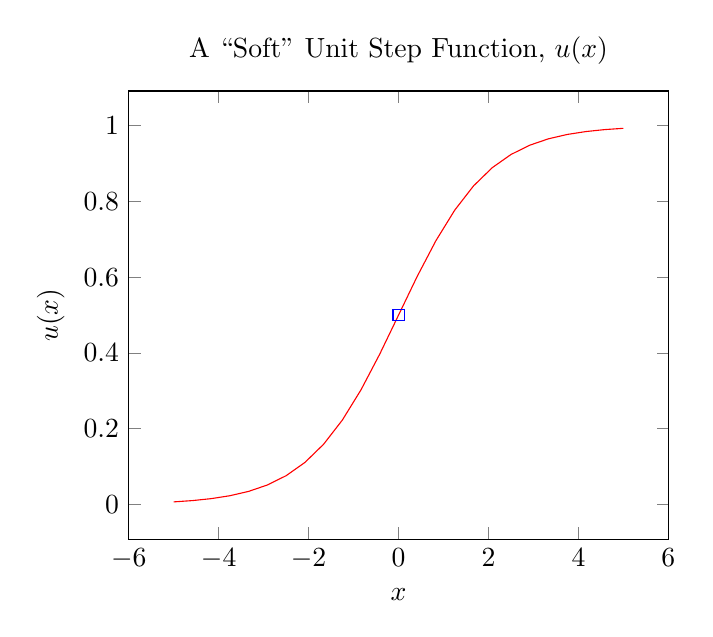
\begin{tikzpicture}
\begin{axis}[
title={A ``Soft" Unit Step Function, $u(x)$},
    xlabel={$x$},
    ylabel={$u(x)$}]
\addplot[color=red]{1/(1 + exp(-x))};
\addplot[
    color=blue,
    mark=square,
    ]
    coordinates {
    (0,0.5)
    };
\end{axis}
\end{tikzpicture}
\end{center}
The gradient of this brightness across the edge, given by $\nabla u(x)$ (or $\der{u}{x}$ in one dimension), is then given by the following.  Notice that the location of the maximum matches the inflection point in the graph above:
\begin{center}
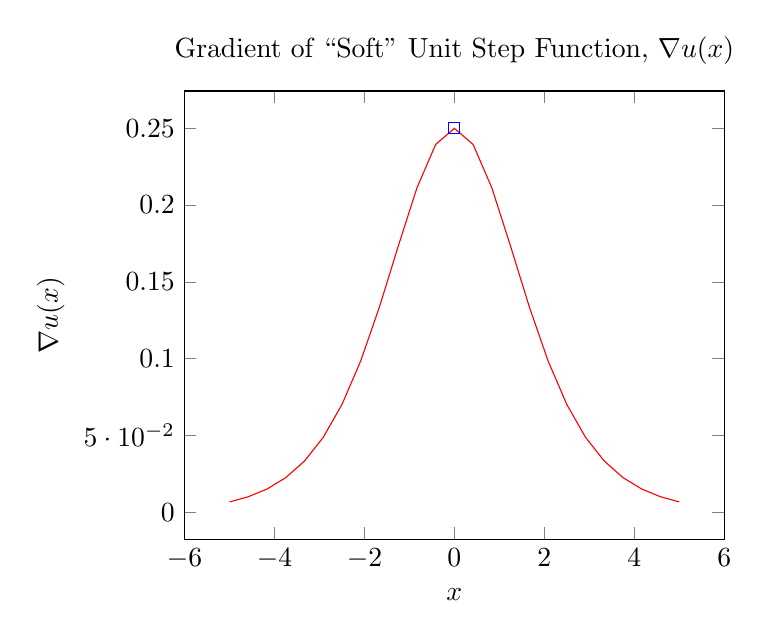
\begin{tikzpicture}
\begin{axis}[
title={Gradient of ``Soft" Unit Step Function, $\nabla u(x)$},
    xlabel={$ x$},
    ylabel={$\nabla u(x)$}]
\addplot[color=red]{exp(-x)/(1 + exp(-x))^2};
\addplot[
    color=blue,
    mark=square,
    ]
    coordinates {
    (0,0.25)
    };
\end{axis}
\end{tikzpicture}
\end{center}
As we mentioned above, we can find the location of this edge by looking at where the second derivative of brightness crosses zero, a.k.a. where $\nabla (\nabla u(x)) = \nabla^2 u(x) = 0$.  Notice that the location of this zero is given by the same location as the inflection point of $u(x)$ and the maximum of $\nabla u(x)$:
\begin{center}
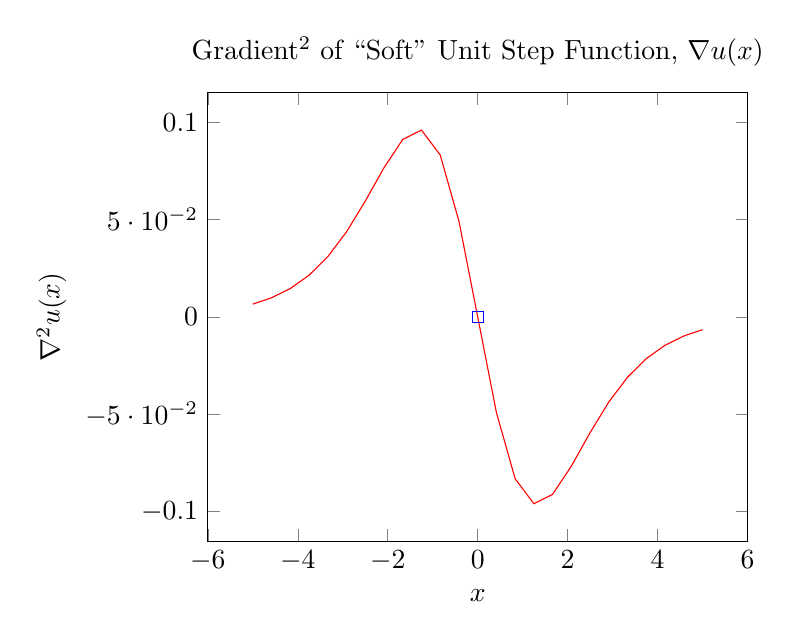
\begin{tikzpicture}
\begin{axis}[
title={Gradient$^2$ of ``Soft" Unit Step Function, $\nabla u(x)$},
    xlabel={$x$},
    ylabel={$\nabla^2 u(x)$}]
\addplot[color=red]{(-exp(-x)*(1+exp(-x))^2 + exp(-x)*2*(1+exp(-x))*exp(-x))/(1+exp(-x))^4};
\addplot[
    color=blue,
    mark=square,
    ]
    coordinates {
    (0,0.0)
    };
\end{axis}
\end{tikzpicture}
\end{center}
For those curious, here is the math behind this specific function, assuming a sigmoid for $u(x)$:
\begin{enumerate}
    \item $u(x) = \frac{1}{1 + \exp{(-x)}}$
    \item $\nabla u(x) = \der{u}{x} = \frac{d}{dx}\Big(\frac{1}{1 + \exp{-x}}\Big) = \frac{\exp(-x)}{(1 + \exp(-x))^2}$
    \item $\nabla^2 u(x) = \dder{u}{x} = \frac{d}{dx}(\frac{\exp(-x)}{(1 + \exp(-x))^2}) = \frac{-\exp(-x)(1+\exp(-x))^2 + 2\exp(-x)(1+\exp(-x))\exp(-x)}{(1+\exp(-x))^4}$
\end{enumerate}
Building on top of this framework above, let us now move on to brightness gradient estimation.
\subsubsection{Brightness Gradient Estimation}
This component of this studied edge detection framework estimates the magnitude and direction of the brightness gradient.  Let us look at how this is derived for different filters: \\ \\
\textbf{Robert's Cross Gradient}: Since this estimates derivatives at 45 degree angles, the pixels are effectively further apart, and this means there will be a constant of proportionality difference between the magnitude of the gradient estimated here and with a normal $(x, y)$ coordinate system:
\begin{align*}
    \sqrt{E^{2}_{x'} + E^{2}_{y'}} \propto \sqrt{E^2_x + E^2_y} &&
\end{align*}
Next, we will look at the Sobel operator.  For this analysis, it will be helpful to recall the following result from Taylor Series:
\begin{align*}
    f(x+\delta x) = f(x) + \delta xf'(x) + \frac{(\delta x)^2}{2!}f''(x) + \frac{(\delta x)^3}{3!}f'''(x) + \frac{(\delta x)^4}{24}f^{(4)}(x) + ... = \sum_{i=0}^{\infty}\frac{(\delta x)^if^{(i)}(x)}{i!}, \;\;\text{where} \; 0! \delteq 1 &&
\end{align*}
Let us first consider the simple two-pixel difference operator (in the x-direction/in the one-dimensional case), \\ i.e. $\der{E}{x} \rightarrow K_x = \frac{1}{\delta}(-1 \; 1)$.  Let us look at the \textbf{forward difference} and \textbf{backward difference} when this operator is applied:
\begin{enumerate}
    \item \textbf{Forward Difference}: $\pd{E}{x} \approx \frac{f(x+\delta x)-f(x)}{\delta x} = f'(x) + \frac{\delta x}{2}f''(x) + \frac{(\delta x)^2}{6}f'''(x) + ...$
    \item \textbf{Backward Difference}: $\pd{E}{x} \approx \frac{f(x)-f(x-\delta x)}{\delta x} = -f'(x) - \frac{\delta x}{2}f''(x) + \frac{(\delta x)^2}{6}f'''(x) + ...$
\end{enumerate}
Notice that for both of these, if $f''(x)$ is large, i.e. if $f(x)$ is nonlinear, then we will have second-order error terms that appear in our estimates.  In general, we want to aim for removing these lower-order error terms.  If we average the forward and backward differences, however, we can see that these second-order error terms disappear:
\begin{align*}
    \frac{\frac{f(x+\delta x)-f(x)}{\delta x} + \frac{f(x)-f(x-\delta x)}{\delta x}}{2} = f'(x) + \frac{(\delta x)^2}{6}f'''(x) + ... &&
\end{align*}
Now we have increased the error term to 3rd order, rather than 2nd order!  As a computational molecule, this higher-order filter Sobel operator looks like $\der{E}{x} \rightarrow K_x = \frac{1}{2\delta}(-1 \; 0 \; 1)$.  But we can do even better!  So long as we do not need to have a pixel at our proposed edge, we can use a filter of three elements spanning $(x-\frac{\delta}{2} \; x \; x + \frac{\delta}{2})$.  There is no pixel at $x$ but we can still compute the derivative here.  This yields an error that is 0.25 the error above due to the fact that our pixels are $\frac{\delta}{2}$ apart, as opposed to $\delta$ apart:
\begin{align*}
    \text{error} = \frac{(\frac{x\delta}{2})^2}{6}f'''(x) &&
\end{align*}
This makes sense intuitively, because the closer together a set of gradient estimates are, the more accurate they will be.  We can incorporate $y$ into the picture, making this amenable for two-dimensional methods as desired, by simply taking the center of four pixels, given for each dimension as:
\begin{align*}
    & \pd{E}{x} \approx K_x = \frac{1}{2\delta_x}\begin{bmatrix}-1 & 1 \\ -1 & 1\end{bmatrix} \\
    & \pd{E}{y} \approx K_y = \frac{1}{2\delta_y}\begin{bmatrix}-1 & -1 \\ 1 & 1\end{bmatrix} &&
\end{align*}
The proposed edge is in the middle of both of these kernels, as shown below:
\begin{figure}[H]
    \centering
    \includegraphics[width=6cm]{figures/xy_filters.png}
    \caption{We can estimate the brightness gradient with minimal error by estimating it at the point at the center of these 2D filters.}
    \label{fig:my_label}
\end{figure}
Estimating these individually in each dimension requires 3 operations each for a total of 6 operations, but if we are able to take the common operations from each and combine them either by addition or subtraction, this only requires 4 operations.  Helpful especially for images with lots of pixels. \\ \\
Next, we will discuss the 3-by-3 Sobel operator.  We can think of this Sobel operator (in each dimension) as being the discrete convolution of a 2-by-2 horizontal or vertical highpass/edge filer with a smoothing or averaging filter:
\begin{enumerate}
    \item \textbf{x-direction}: $\frac{1}{2\delta_x}\begin{bmatrix}-1 & 1 \\ -1 & 1\end{bmatrix} * \begin{bmatrix}1 & 1 \\ 1 & 1\end{bmatrix} = 
    \begin{bmatrix}-1 & 0 & 1 \\ -2 & 0 & 2 \\ -1 & 0 & 1 \end{bmatrix}$
    \item \textbf{y-direction}: $\frac{1}{2\delta_y}\begin{bmatrix}-1 & -1 \\ 1 & 1\end{bmatrix} * \begin{bmatrix}1 & 1 \\ 1 & 1\end{bmatrix} = 
    \begin{bmatrix}-1 & -2 & -1 \\ 0 & 0 & 0 \\ 1 & 2 & 1 \end{bmatrix}$
\end{enumerate}
A few notes about the derivation above:
\begin{itemize}
    \item The convolution used is a ``padded convolution" [3], in which, when implemented, when the elements of the filter/kernel (in this case, the averaging kernel) are not aligned with the image, they are simply multiplied by zero.  Zero padding is the most common padding technique, but there are other techniques as well, such as wraparound padding.
    \item This approach avoids the half-pixel (in which we estimate an edge that is not on a pixel) that was cited above.
    \item Smoothing/averaging is a double edge sword, because while it can reduce/remove high-frequency noise by filtering, it can also introduce undesirable blurring.
\end{itemize}
Next, we will look at how the brightness gradient is converted from Cartesian to Polar coordinates:
\begin{align*}
    & (E_x, E_y) \rightarrow (E_0, E_{\theta}) \\
    & E_0 = \sqrt{E^2_x + E^2_y} \\
    & E_{\theta} = \tan^{-1}\Big(\frac{E_y}{E_y}\Big) &&
\end{align*}
Finally, we conclude this lecture by looking at appropriate values of $s$ for quadratic and triangular functions.  This assumes we have three gradient measurements centered on $G_0$: (1) $G_{-}$, (2) $G_0$, and (3) $G_{+}$.  Let us look at the results for these two types of functions:
\begin{enumerate}
    \item \textbf{Quadratic}: $s = \frac{G_{+} - G_{-}}{4(G_0 - \frac{1}{2}(G_{+}-G_{-}))}$, this results in $s \in [-\frac{1}{2}, \frac{1}{2}]$.
    \item \textbf{Triangular}: $s = \frac{G_{+} - G_{-}}{2(G_0 - \min(G_{+}, G_{-}))}$
\end{enumerate}
A few notes about these approaches:
\begin{itemize}
    \item Note that in each case, we only want to keep if the magnitude $G_0$ is a local maximum, i.e. $G_0 > G_{+}$ and $G_0 \geq G_{-}$.
    \item In the quadratic case, we can parameterize the curve with three data points using three degrees of freedom, i.e. $ax^2 + bx + c = 0$.  With this approach, $b \approx \text{first derivative}$ and $a \approx \text{second derivative}$.
\end{itemize}
\subsection{References}
\begin{enumerate}
    \item CORDIC Algorithm, https://www.allaboutcircuits.com/technical-articles/an-introduction-to-the-cordic-algorithm/
    \item Non-Maximum Supression, http://justin-liang.com/tutorials/canny/\#suppression
    \item Padded Convolution, https://medium.com/@ayeshmanthaperera/what-is-padding-in-cnns-71b21fb0dd7
\end{enumerate}
\end{document} 